\subsubsection{\bf Introduction}
LineTrackingMonitor is a tool to monitor various lines included in the strain data.
The amplitude and frequency are tracked.


\subsubsection{{\bf Function:} butterBandPass}
{\tt ~ butterBandPass dat fs flow fhigh order\\}
This applies a Butterworth bandpass filter of given cutoff frequencies and filter order to given data.

The arguments are:
\begin{itemize}
\item {\tt dat}: Input. data
\item {\tt fs}: Input. Sampling frequency [Hz]
\item {\tt flow}: Input. Lower cutoff frequency [Hz]
\item {\tt fhigh}: Input. Higher cutoff frequency [Hz]
\item {\tt order}: Input. Filter order
\end{itemize}

It should be noted that this filter is a zero-phase filter (so called filtfilt), so the effective filter order is twice your input value (For example, if you set order $= 5$, the actual filter order becomes ten).


\subsubsection{{\bf Function:} nha}
{\tt ~ nha dat fs nsig nframe nshift nstart nend tlength\\}


The arguments are:
\begin{itemize}
\item {\tt dat}: Input.
\item {\tt fs}: Input. Sampling frequency [Hz]
\item {\tt nsig}: Input. The number of signals (lines) to extract
\item {\tt nframe}: Input. Frame length
\item {\tt nshift}: Input. Shift length
\item {\tt nstart}: Input. The start point
\item {\tt nend}: Input. The end point
\item {\tt tlength}: Input. Time length of data
\end{itemize}


\subsubsection{Sample plots of LineTrackingMonitor}

\begin{figure}[t]
 \begin{center}
    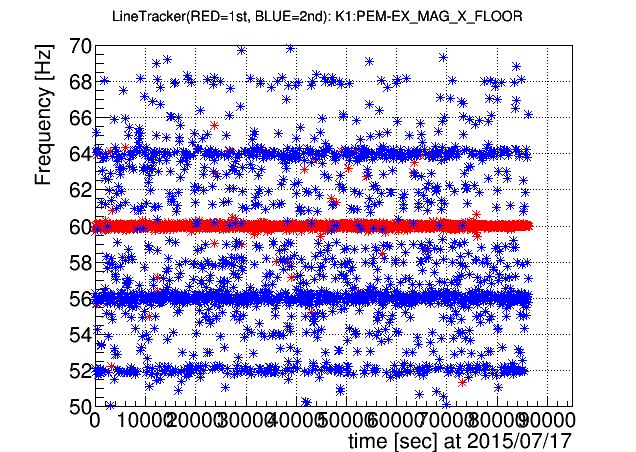
\includegraphics[width=0.9\hsize]{fig/LineTrackingMon/sample_freq.png}
    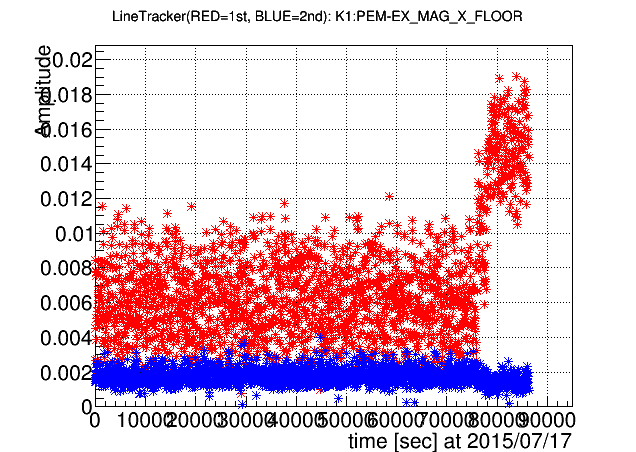
\includegraphics[width=0.9\hsize]{fig/LineTrackingMon/sample_amp.png}
    \caption{sample plots of frequency (top) and amplitude (bottom) of LineTrackingMonitor}
 \end{center}
\end{figure}

{\noindent \small contact person: Koh Ueno (\tt ueno@gwv.hep.osaka-cu.ac.jp)}

